\documentclass[10pt,twocolumn,letterpaper]{article}

\usepackage{cvpr}
\usepackage{times}
\usepackage{epsfig}
\usepackage{graphicx}
\usepackage{amsmath}
\usepackage{amssymb}
\usepackage{kotex}

% Include other packages here, before hyperref.

% If you comment hyperref and then uncomment it, you should delete
% egpaper.aux before re-running latex.  (Or just hit 'q' on the first latex
% run, let it finish, and you should be clear).
\usepackage[breaklinks=true,bookmarks=false]{hyperref}

\cvprfinalcopy % *** Uncomment this line for the final submission

\def\cvprPaperID{****} % *** Enter the CVPR Paper ID here
\def\httilde{\mbox{\tt\raisebox{-.5ex}{\symbol{126}}}}

% Pages are numbered in submission mode, and unnumbered in camera-ready
%\ifcvprfinal\pagestyle{empty}\fi
\setcounter{page}{1}
\begin{document}

%%%%%%%%% TITLE
\title{PROJECT2. Human Action Recognition using Hidden Markov Model}

\author{Sangjun Son\\
Seoul National University\\
Department of Computer Science and Engineering\\
{\tt\small lucetre@snu.ac.kr}
}

\maketitle

\section{Introduction}

Hidden Markov Model has such a good strength in analyzing sequential data, and had been widely used in language model, part-of-speech tagging and named entity recognition \cite{ratgo}. Based on Markov process, HMM infers probability distributions of the model from observations and find the most likely results so far. It is useful for cases unable to observe all datasets and only able to get its causal evidences, and can be applied in many different data restoring fields \cite{wikipedia}, e.g. multiple DNA sequence alignment, protein secondary structure prediction \cite{biology} and speech recognition. Datasets being used in HMM modeling should be time-serial. For example, speech recognition has temporal structure consisted of statistical models and can be encoded as a sequence of spectral vectors spanning the audio frequency range \cite{speechrecognition}.

Likewise, we'd like to use temporal human action sensor data to make Human Action Recognition system (HAR) using HMM. We've trained our model with  Human Activities and Postural Transitions datasets (HAPT) produced by Jorge L, \etal \cite{hapt}. Measurement was done by 30 volunteers carrying a waist-mounted smartphone with embedded inertial sensors. Dataset includes 61 experiments with 30 participants and measured in 50Hz frequency and about 400s duration per experiment. Each experiment contains 12 types of human actions like standing, walking down, \etc. We separated into 12 part of data so we can easily train our model by action type. Eventually, we've got 1,214 examples and randomly splitted as train and test dataset as 9:1 ratio respectively.

%-------------------------------------------------------------------------
\section{Related Works}
Human activity recognition is nowadays an active research field which aims to understand human behavior and there have been lots of researches to figure out human behaviours. One of the approaches was method consisted of support vector machines (SVMs) and temporal filters of activity probability estimations within a limited time window \cite{haptpaper}. Probability estimation after feature extraction was done by MAP filtering.

Rubén San-Segundo, \etal have implemented system comprising of three main modules: feature extraction, HMMs training and activity recognition. In the training module, 6 HMM modules were being trained to classify human actions with datasets of only six different physical activity types: walking, walking-upstairs, walking-downstairs, sitting, standing and lying down. Due to the lack amount of activity types they've obtained the recognition error rate of 2.5\% \cite{monitoring}.

%-------------------------------------------------------------------------
\section{Preliminaries}

\section{Hidden Markov Model}

\begin{center}
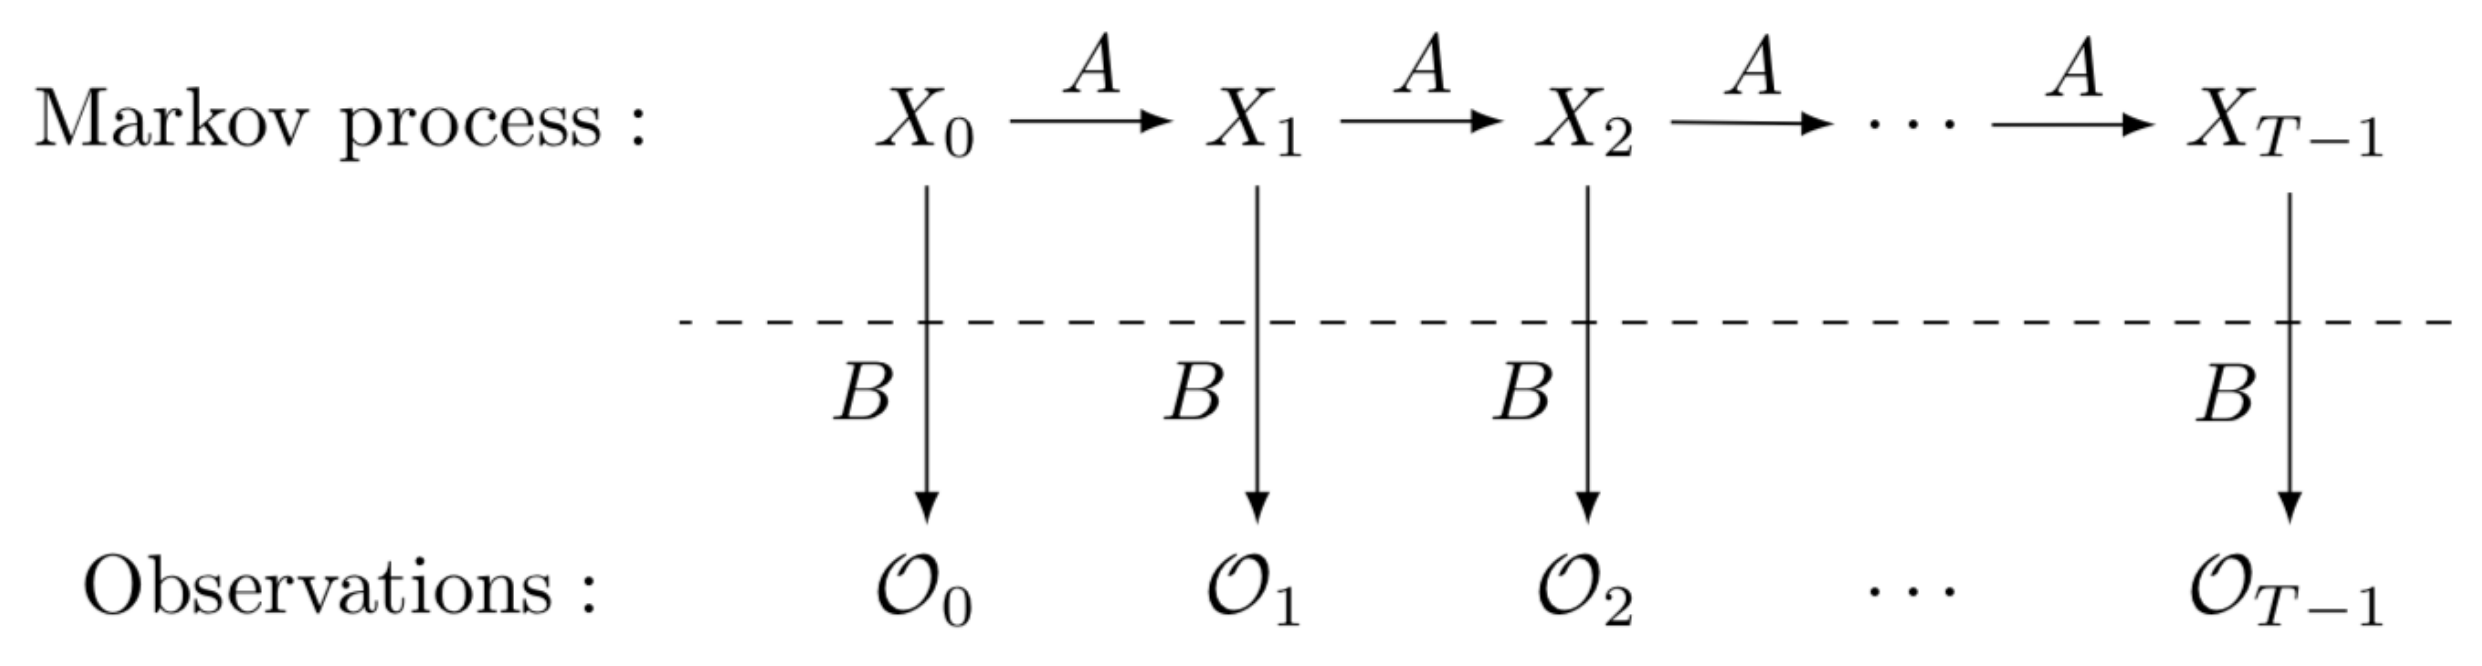
\includegraphics[width=1.0\linewidth]{./HMM.png}
\end{center}

A hidden Markov model (HMM) allows us to talk about both observed events (like words that we see in the input) and hidden events (like part-of-speech tags) that we think of as causal factors in our probabilistic model. HMM model $\lambda$ contains transition probability matrix $A$, a set of state variables $X$, a sequence of observations $O$, emission probabilities $B$, and an initial probability distribution over states $\pi$.

We can characterized HMM into 3 fundamental problems;

1. Given the model $\lambda$, we have to find likelihood $P(O|\lambda)$ whether the observation $O$ is a probable sequence based on $\lambda$.
2. Given an observation sequenceOand an HMMλ=(A,B), discover the best hidden state sequenceQ.

%-------------------------------------------------------------------------
\section{Proposed Method}

%-------------------------------------------------------------------------
\section{Empirical Analysis}

%-------------------------------------------------------------------------
\section{Conclusion}


\begin{thebibliography}{9}

\bibitem{ratgo} 
ratgo’s blog

\bibitem{wikipedia} 
Wikipedia, Hidden Markov model

\bibitem{biology} 
Byung-Jun Yoon, 
``Hidden Markov Models and their Applications in Biological Sequence Analysis"

\bibitem{speechrecognition} 
M. Gales and S. Young
``The Application of Hidden Markov Models in Speech Recognition".
{\textit{Foundations and Trends in Signal Processing, Vol.1, No.3}, 2007}

\bibitem{hapt}
Jorge L. Reyes-Ortiz, Davide Anguita, Alessandro Ghio, Luca Oneto and Xavier Parra,
``Smartphone-Based Recognition of Human Activities and Postural Transitions Data Set"
, 2015

\bibitem{haptpaper}
Jorge L, \etal
``Human Activity Recognition on Smartphones with Awareness of Basic Activities and Postural Transitions"
{\textit{ICANN 2014, LNCS 8681, pp.177–185}, 2014}

\bibitem{monitoring}
Rubén San-Segundo, Julián David Echeverry-Correa, Christian Salamea, José Manuel Pardo
``Human activity monitoring based on hidden Markov models using a smartphone"
{\textit{IEEE Instrumentation and Measurement Magazine}, 2016}

\end{thebibliography}

% [4] B.H. Williams, M.Toussaint, and A.J. Storkey. Extracting motion primitives from natural handwriting data. In ICANN, volume 2, pages 634–643, 2006.
% [5] UCI Machine Learning Repository, Character Trajectories Data Set
% [6] Chun Yuan. et al, A Handwritten Character Recognition System Based on Acceleration, January 2011
% [7] API Documentation of sklearn.model_selection.train_test_split (https://scikit-learn.org/stable/modules/generated/sklearn.model_selection.train_test_split.html)
% [8] API Documentation of hmmlearn.MultinomialHMM (https://hmmlearn.readthedocs.io/en/latest/api.html#multinomialhmm)

\end{document}
